\chapter{Fundamentação Teórica}
\label{chap:fundamentacao}

Este capítulo apresenta uma breve introdução sobre os conceitos utilizados neste
trabalho. Primeiro, são abordadas as partes do \textit{pipeline} de um compilador
de maneira a entender, ao menos superficialmente, os passos de compilação.
Em seguida, discute-se como o compilador GCC apresenta esses tópicos implementados,
além do seu uso clássico do processo de compilação de um programa. Por fim, são
apresentados alguns conceitos e algoritmos básicos sobre Computação Paralela.
%tá lindo

\begin{section}{Compiladores}

Para evitar confusões a respeito das diferentes linguagens que um compilador
trabalha em seus muitos estágios, vamos adotar a seguinte nomenclatura:
Denote \textit{Linguagem Fonte} como sendo a linguagem
na qual o código fonte do programa a ser compilado foi originalmente escrito;
\textit{Linguagem Intermediária} uma das linguagens internas do compilador; e
\textit{Linguagem Alvo} a linguagem na qual o compilador deverá gerar código.

Compiladores são grandes projetos destinados a tradução de códigos fonte
entre distintas linguagens de programação. Normalmente, compiladores traduzem
linguagens de alto nível, como C, para linguagens mais próximas da máquina,
como a linguagem de montagem - embora isso não seja uma regra pois existem
compiladores cuja única tarefa é realizar uma tradução entre duas linguagens
de alto nível.

Compiladores também costumam otimizar
o código que passam por eles, aplicando diversas heurísticas de
maneira a acelerar o código a ser produzido, substituindo trechos de código por
outros mais eficientes, reordenando as instruções do programa, etc.

Por serem programas extremamente grandes, existe um grande interesse em evitar
reescrever um novo compilador
sempre que uma nova linguagem é proposta, ou um novo \textit{hardware} é criado.
Para isso, a seguinte modularização é largamente adotada por projetistas de
compiladores \citep{redhat} \citep{llvm}, conforme ilustrado na Figura \ref{fig:compiler_arch}:

\begin{itemize}
    \item Um \textit{Front End} para cada Linguagem Fonte.
	Neste módulo são executadas as análises léxica e sintática, com a
        finalidade de construir uma Árvore de Sintaxe Abstrata(AST), para que, em
seguida, ela seja convertida para uma Linguagem Intermediária do compilador.

    \item Um \textit{Middle End}, responsável por aplicar diversas otimizações
independentes de arquitetura no código já convertido para a Linguagem Intermediária.

    \item Um \textit{Back End} para cada linguagem alvo, responsável por converter a linguagem intermediária
na linguagem alvo. Aqui outras otimizações específicas da linguagem alvo são realizadas,
como alocação de registradores.

\end{itemize}

Porém, essa modularização é opcional: compiladores mais antigos destinados a fazer uma
conversão direta entre duas linguagens, como o UNIX C Compiler, não costumam usar uma linguagem
intermediária \citep{ritchie1979tour}, além de diversos livros-texto não mencionarem tal módulo, fundindo suas
funcionalidades com o \textit{Front End} \citep{dragonbook}. Não adotar tal metodologia
simplifica o projeto, mas dificulta a inserção de suporte a novas
linguagens de programação.


\begin{figure}
\tikzstyle{block} = [rectangle, draw, fill=white,
    text width=6em, text centered, rounded corners, node distance=5cm, auto, minimum height=2em]
\tikzstyle{line} = [draw, -latex]
\tikzstyle{cloud} = [draw, ellipse,fill=white, node distance=2cm,
    minimum height=2em]

\begin{center}
\scalebox{0.8}{
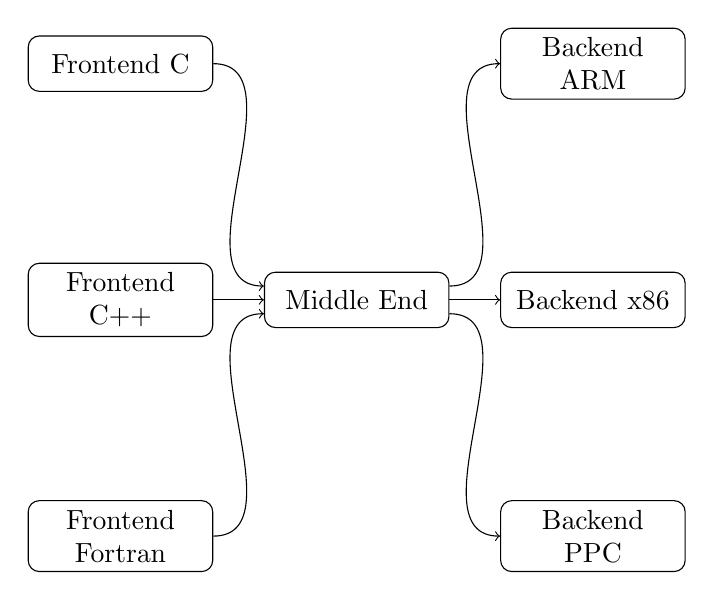
\begin{tikzpicture}[node distance = 3cm, auto]
    % Place nodes
    \node [block]                      (front_c)    {Frontend C};
    \node [block, below of=front_c]    (front_cpp)  {Frontend C++};
    \node [block, below of=front_cpp]  (front_fort) {Frontend Fortran};
    \node [block, right of=front_cpp]  (middle)     {Middle End};
    \node [block, right of=middle]     (back_x86)   {Backend x86};
    \node [block, above of=back_x86]   (back_arm)   {Backend ARM};
    \node [block, below of=back_x86]   (back_ppc)   {Backend PPC};


    \coordinate [left of=front_c]    (c_code);
    \coordinate [left of=front_cpp]  (cpp_code);
    \coordinate [left of=front_fort]  (fort_code);

    \coordinate [right of=back_x86] (x86_code);
    \coordinate [right of=back_arm] (arm_code);
    \coordinate [right of=back_ppc] (ppc_code);

    % Draw edges
    \draw[->]    (front_c.east)     to [out=0,in=180] ([yshift=0.5em]  middle.west);
    \draw[->]    (front_cpp.east)   to [out=0,in=180] (middle.west);
    \draw[->]    (front_fort.east)  to [out=0,in=180] ([yshift=-0.5em] middle.west);

    \draw[->]    ([yshift=-0.5em] middle.east)  to [out=0,in=180] (back_ppc.west);
    \draw[->]    (middle.east)                  to [out=0,in=180] (back_x86.west);
    \draw[->]    ([yshift=0.5em] middle.east)   to [out=0,in=180] (back_arm.west);

    %\draw[->]    (sintatico.west)   -- (lexico.east)    node[midway] {próximo\_token()};
    %\draw[->]    (fonte.west)       -- (lexico.west)    node[pos=0, above] {Código Fonte};
    %\draw[->]    (sintatico.east)   -- (ast.west)       node[pos=1, above] {Árvore Abstrata};
\end{tikzpicture}
}
\end{center}

\caption{Arquitetura de um compilador.}
\label{fig:compiler_arch}
\end{figure}

\begin{subsection}{\textit{Front End}}

Um \textit{Front End} é um módulo responsável por interagir diretamente com o
código escrito na Linguagem Fonte a ser compilado. Ele costuma ser único
para cada Linguagem Fonte, ou seja, para inserir suporte a uma nova
Linguagem Alvo, basta implementar um novo \textit{Front End}, mas é 
possível que algumas classes sejam
compartilhadas, como no caso de um compilador que dê suporte tanto para C quanto para C++. 


Como primeiro passo, \textit {Front End} realiza uma análise
léxica e sintática, com a finalidade de gerar uma AST e verificar
se o texto dado como entrada realmente pertence à linguagem.
Estes dois analisadores se comunicam constantemente, conforme ilustrado na Figura
\ref{fig:lexico_sintatico}.


\begin{figure}
\tikzstyle{block} = [rectangle, draw, fill=white,
    text width=6em, text centered, rounded corners, node distance=9cm, auto, minimum height=2em]
\tikzstyle{line} = [draw, -latex]
\tikzstyle{cloud} = [draw, ellipse,fill=white, node distance=2cm,
    minimum height=2em]

\begin{center}
\scalebox{0.8}{
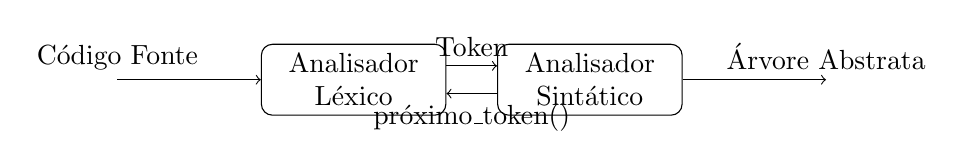
\begin{tikzpicture}[node distance = 3cm, auto]
    % Place nodes
    \node [block]                    (lexico) {Analisador Léxico};
    \node [block, right of = lexico] (sintatico) {Analisador Sintático};
    \coordinate [left of=lexico]     (fonte);
    \coordinate [right of=sintatico] (ast);

    % Draw edges
    \draw[->]    ([yshift=0.5em] lexico.east)       -- ([yshift=0.5em] sintatico.west) node[midway] {Token};
    \draw[->]    ([yshift=-0.5em] sintatico.west)   -- ([yshift=-0.5em] lexico.east)    node[midway] {próximo\_token()};
    \draw[->]    (fonte.west)                       -- (lexico.west)    node[pos=0, above] {Código Fonte};
    \draw[->]    (sintatico.east)                   -- (ast.west)   node[pos=1, above] {Árvore Abstrata};
\end{tikzpicture}
}
\end{center}

\caption{Interações entre um analisador léxico e sintático.}
\label{fig:lexico_sintatico}
\end{figure}

    Primeiro, a análise léxica é responsável por ler o arquivo
de texto contendo o código fonte, e quebrar as palavras em \textit{tokens}, que
serão alimentados para o analisador sintático. Por consequência, ele é capaz de
realizar alguns filtros, \textit{e.g}. ignorar os comentários, identificar constantes
numéricas, eliminar espaços desnecessários, e substituir um \textit{token} por
outro.
Analisadores léxicos também podem ser usados para substituição
de macros, como implementado pelo preprocessador do C
(CPP)\footnote{https://gcc.gnu.org/onlinedocs/cppinternals/Lexer.html}.

Geralmente, os Analisadores Léxicos são implementados utilizando autômatos
por diversos motivos, entre eles sua atrativa complexidade computacional
$O(n)$, onde $n$ é o tamanho da entrada, pela existência de algoritmos
para converter expressões regulares em autômatos \citep{thompson}, e pela
existência de algoritmos para minimização de estados de um autômato
\citep{hopcroft1971n}. Isto possibilita que geradores de analisadores léxicos
como o \texttt{Flex}\footnote{https://www.gnu.org/software/flex/}
sejam bastante eficientes.

    Em sequência, o Analisador Sintático entra em cena. O analisador sintático é
responsável por gerar a Árvore de Sintaxe Abstrata (AST), inspecionando a
sequência de \textit{tokens} fornecida pelo Analisador Léxico. Neste processo,
ele certifica-se de que o código fonte respeita a gramática da linguagem,
apontando erros caso contrário.

    Analisadores Sintáticos se apoiam nas gramáticas não ambíguas que geram uma
linguagem livre de contexto determinística, isto porque gramáticas mais
poderosas requerem algoritmos computacionalmente mais custosos
\citep{sipser2012}. Existem vários algoritmos para realizar a análise sintática,
mas destacam-se:
\begin{itemize}
	\item Recursivo Descendente: Um algoritmo de caráter preditivo, que tenta
	    construir a AST da raiz para as folhas. Uma característica desse algoritmo
		é a sua facilidade de codificação, que utiliza chamadas de funções para
		armazenar o contexto atual e progredir na análise conforme as regras da
		gramática. Seu uso é devido a facilidade de codificação e mensagens de
		erro mais informativas para o usuário.

    \item LL($k$): Outro algoritmo de caráter preditivo, que tenta construir a AST da
        raiz para as folhas. Aqui o algoritmo usa uma máquina de estados em conjunto
		com uma pilha para armazenar o contexto atual. Sua codificação é mais
		complexa que o anterior, e as mensagens de erro costumam ser mais precárias.

    \item LR($k$): Um algoritmo que tenta construir a AST das folhas para a raiz.
		  Assim como o LL($k$), este algoritmo também utiliza uma máquina de estados
		  em conjunto com uma pilha. Apesar de sua codificação ser mais complicada,
          esse algoritmo consegue processar gramáticas mais complexas que
          o LL($k$), conforme proposto por \cite{knuth1965translation}. 
          Outra vantagem interessante é a existência de
          \textit{softwares} como o
          \texttt{Bison}\footnote{https://www.gnu.org/software/bison/}, capaz
          de gerar um analisador LR($1$) a partir da especificação da gramática.
\end{itemize}
	A complexidade dos analisadores LL($k$) e LR($k$) é $O(n)$, onde $n$ 
	é o tamanho da entrada. Já o Recursivo Descendente a complexidade pode variar
	dependendo da implementação.
    Por fim, uma descrição mais detalhada do funcionamento destes algoritmos
pode ser encontrada em \citep{appel2004modern}.

    Uma vez gerada a AST, é possível fazer verificações extras de semântica
relacionada a linguagem de programação. Em seguida, essa AST normalmente é
traduzida para uma linguagem intermediária, onde serão feitas otimizações
independentes da linguagem alvo no código. Por fim, o controle é passado
para o \textit{Middle End} do compilador.

\end{subsection}

\begin{subsection}{\textit{Middle End}}

    O \textit{Middle End} é responsável por trabalhar em uma ou mais
 Linguagens Intermediárias do compilador, com a finalidade de efetuar
otimizações no código e possíveis checagens de erro que possam ser
postergadas até essa fase. Essas linguagens devem ser projetadas
de maneira a capturar a semântica da Linguagem Fonte, na qual o programa original foi
escrito.
Existem várias representações convenientes para a Linguagem Intermediária,
mas destaca-se para fins de otimização
a \textit{Three-Address Code}, que normalmente é usada em conjunto com
a \textit{Static Single Assignment} (SSA).

\begin{subsubsection}{\textit{Three-Address Code}}

Nesta representação, expressões como $a*x + b$ são
representadas como:
$$ t_1 = a*x$$
\vspace*{-1cm}
$$ t_2 = t_1 + b $$
ou seja, todas as expressões são transformadas em uma sequência de expressões
contendo apenas dois operandos e uma operação de atribuição. Para isso,
novas variáveis são declaradas para conter os valores intermediários
possibilitando também a remoção de sub-expressões em comum. Também nesta
linguagem, fluxo de código e laços são transformados em uma sequência de
\texttt{if} e \texttt{goto} para facilitar a construção de um grafo de
controle de fluxo, possibilitando análises nessa estrutura.
Esta representação é demasiada útil por facilitar o processo de alocação
de registradores, uma vez que nela, a maneira de como os processadores
operam instruções aritméticas é representada com fidelidade\citep{lattner2002llvm}.

\end{subsubsection}
\begin{subsubsection}{\textit{Static Single Assignment}}

O \textit{Static Single Assignment} (SSA) é uma linguagem intermediária
onde uma variável é atribuída uma única vez. Sendo assim, toda vez que
uma variável no código original é modificada, é necessário criar na representação SSA uma
nova variável para registrar essa atribuição. Isto facilita diversas
otimizações no controle de fluxo do programa, assim como possibilita a remoção
de variáveis não utilizadas ou que não serão mais utilizadas em um
trecho de código, processo conhecido como \textit{Liveness Analysis}.

\vspace*{-0.5cm}
Entretanto, quando essa representação é
    usada em conjunto com um fluxo de execução, como \texttt{if-else}, isso pode gerar um problema. Considere o código
na Figura \ref{fig:code_normal}. Neste código há dois valores possíveis para
$a$ quando a expressão $u = a*v$ for executada, sendo necessário
anotar qual versão de $a$ utilizar. A solução é introduzir uma
função $\phi$, que seleciona a variável corretamente utilizando a informação
do arco usado para se chegar no bloco contendo a sentença com a função $\phi$,
conforme ilustrado na Figura \ref{fig:code_ssa_form}.

\begin{figure}[ht]
    \centering
    \begin{subfigure}[b]{0.40\textwidth}

        \begin{lstlisting}[
            language=pseudocode,
            style=pseudocode,
            style=wider,
            functions={},
            specialidentifiers={extern, call},
            ]
            if (condition) then
                a = -1;
            else
                a = 1;
            end
            u = a*v;
        \end{lstlisting}
        \caption{\label{fig:code_normal}}
    \end{subfigure}
    \begin{subfigure}[b]{0.40\textwidth}
        \begin{lstlisting}[
                language=pseudocode,
                style=pseudocode,
                style=wider,
                functions={},
                specialidentifiers={extern, call, PHI},
              ]
            if (condition) then
                $a_1$ = -1;
            else
                $a_2$ = 1;
            end
            $a_3$ = $\phi$($a_1$, $a_2$)
            u = $a_3$*v;
        \end{lstlisting}
        \caption{\label{fig:code_ssa_form}}
\end{subfigure}
\caption{Um programa (a) e sua representação em SSA em (b)}
\end{figure}

Quanto a implementação de SSA em compiladores, \cite{cytron1991efficiently}
discute com detalhes os algoritmos para construir tal representação. Já
\cite{appel2004modern} discute tal representação em alto nível, evidenciando
possíveis otimizações nesta representação.

\end{subsubsection}

\begin{subsubsection}{Otimizações Independente de Arquitetura}

Uma das funcionalidades mais atrativas de um compilador é sua
capacidade de fazer otimizações no código enquanto mantém
a corretude do mesmo, principalmente quando
o alvo é uma linguagem de montagem. Um compilador com essa
funcionalidade é capaz de gerar código que economiza energia
gasta em processamento, poupa esforços de otimização, desenvolvimento,
entre outros.

Considerando o contexto de um compilador capaz de compilar
diversas linguagens para os mais variados alvos, é exatamente
no \textit{Middle End} onde é alocado maior parte do tempo
gasto na implementação de otimizações, pois isto implica gerar um código mais
eficiente para todas as Linguagens Alvo cujo o compilador dê suporte.

Como o \textit{Front End} já traduziu todo o código para a linguagem
intermediária, então é perfeitamente possível marcar o início de
todas as funções do código. Com isto, é possível particionar o
conjunto das possíveis otimizações em dois conjuntos disjuntos:

\begin{itemize}
    \item Otimizações \textit{Intra-Procedurais}: Otimizam cada função sem
interagir com as demais funções do programa.

    \item Otimizações \textit{Inter-Procedurais}: Procuram observar o programa
como um todo, observando as interações de cada função com as demais
funções do programa. Um exemplo clássico é remover funções não utilizadas, e
decidir se uma determinada função será compilada com o atributo \texttt{inline}.
\end{itemize}
Essa distinção é útil pois não há dependência entre as funções
ao aplicar uma otimização \textit{Intra-Procedural}, e portanto as
funções podem ser processadas em paralelo.
Diversas otimizações
clássicas como Invariante de Laços, Propagação de Constantes,
Eliminação de Redundância, Eliminação de Subexpressão Comum,
Propagação de Constantes, e Eliminação de Código Morto são
classificadas como tal, reforçando o argumento de paralelização.

Já esse argumento é válido para as otimizações \textit{Inter-Procedurais}, pela
própria definição. Estas otimizações são normalmente aplicadas
utilizando algoritmos em grafos:
Cada rotina é representado como um vértice, e existe um arco de $f$
à $g$ se $f$ chama $g$ em seu corpo, conforme ilustrado na Figura
\ref{fig:call_graph}. Construir tal grafo pode ser
um desafio dependendo da linguagem de programação, principalmente
quando se utiliza orientação a objetos devido a possibilidade de
sobrescrita de métodos. Por fim, mais detalhes a respeito dos 
algoritmos referentes a essas otimizações são discutidos por
\cite{khedker2009data}.

\begin{figure}[ht]
\centering
  \begin{subfigure}[b]{0.40\textwidth}
    \tikzstyle{line} = [draw, -latex]
    \tikzstyle{node} = [draw, circle]
    \begin{center}
    \scalebox{0.8}{
    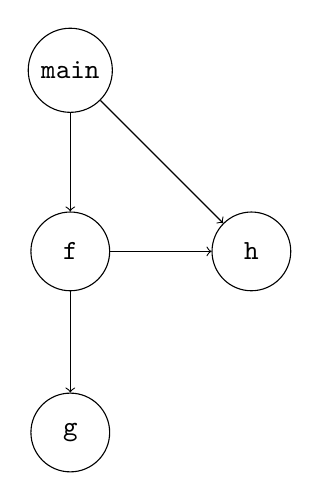
\begin{tikzpicture}[node distance = 2.3cm, minimum height = 1cm, auto]
        % Place nodes
        \node [node]                    (main) {\texttt{main}};
        \node [node, below of = main]        (f) {\texttt{f}};
        \node [node, below of = f]           (g) {\texttt{g}};
        \node [node, right of = f]           (h) {\texttt{h}};

        % Draw edges
        \draw[->]    (main)           -- (f);
        \draw[->]    (f)              -- (g);
        \draw[->]    (f)              -- (h);
        \draw[->]    (main)           -- (h);
    \end{tikzpicture}
    }
    \end{center}
  \end{subfigure}
  \begin{subfigure}[b]{0.40\textwidth}
      \begin{lstlisting}[
        language=pseudocode,
        style=pseudocode,
        style=wider,
        functions={},
        specialidentifiers={extern, call},
      ]
        extern function g,h

        function f()
            call $g$
            call $h$
        end

        function main()
            call $f$
            call $h$
        end
      \end{lstlisting}
  \end{subfigure}
  \caption{Um programa e seu respectivo grafo de chamada de funções}
  \label{fig:call_graph}
\end{figure}


    Após todo esse processo de otimização, o código nesta linguagem ainda
pode ainda sofrer transformações para outras Linguagens
Intermediárias para algo que seja mais próximo do
\textit{hardware}-alvo, no caso da compilação ter como alvo código de máquina.
Finalmente, após essa sequência de transformações, o controle é
passado ao \textit{Back End} do compilador, onde ele será transformado na
Linguagem Alvo.

\end{subsubsection}

\end{subsection}

\begin{subsection}{\textit{Back End}}
    O \textit{Back End} é responsável pela geração do código final na
Linguagem Alvo, além otimizações dependentes
de arquitetura. Sendo assim, ele também deve efetuar otimizações referente
a  seleção de instruções mais eficazes e alocação registradores
da melhor maneira possível para as variáveis do programa, caso a linguagem alvo
seja a Linguagem de Montagem.

    Existem diversas técnicas para selecionar instruções. Uma estratégia possível
é  utilizar uma abordagem de substituição de macros, onde as instruções são substituídas
observando localmente cada linha de código da Linguagem Intermediária. Esta estratégia
tem a vantagem de realizar uma tradução rápida e de fácil implementação, mas que gera
código ineficiente. 

    Outra maneiras incluem identificar padrões a partir de uma árvore
construída, e selecionar a construção que minimiza uma função custo, seja através de uma
heurística, ou usando \textit{Programação Dinâmica}. 

	Também é possível implementar tal tradução utilizando as mesmas técnicas de
análise léxica e sintática empregados no \textit{Front End}, desde que a
Linguagem Intermediária tenha sido projetada considerando tal fato, conforme
sugerido por \cite{glanville1978}. 

Por fim, uma discussão mais detalhada sobre
as técnicas de geração de código de máquina é discutida por
\cite{blindell2016instruction}. Além disso, para 
 adicionar suporte a uma nova arquitetura ou linguagem
alvo, basta implementar um novo \textit{Back End}, aproveitando todo
o código já implementado nas etapas anteriores.
\end{subsection}


\end{section}


\begin{section}{O Compilador GCC}

A coleção de compiladores da GNU, também conhecido como GCC, é um projeto
iniciado por Richard Stallman com a primeira versão disponibilizada ao público
em Março de 1987. Tal versão apenas fornecia suporte a linguagem C, mas já permitia
    gerar código para diversas arquiteturas \citep{gcc_first_ver}.
Hoje, o GCC oferece suporte a diversas Linguagens Fonte como C, C++, Fortran, Go, Ada,
e várias arquiteturas, como i386, amd64, riscv, arm, ppc, pdp-11. O GCC também
é um compilador otimizador, ou seja, ele é capaz de alterar o código fornecido
pelo usuário com a finalidade de gerar código mais eficiente, sem alterar a semântica do programa. Isso é
possível por conta das várias Linguagens Intermediárias implementadas no
GCC. São estas: GENERIC, GIMPLE, e RTL. O compilador executa vários
passos de otimização em cada uma dessas linguagens intermediárias.

\begin{subsection}{GENERIC}

    O GENERIC é uma linguagem intermediária que possibilita representar quaisquer
funções do programa através de árvores. Tal linguagem é um superconjunto
das funcionalidades e atributos que cada Linguagem Fonte contém, por exemplo, atributos
como \texttt{volatile} de C e C++ contém uma representação nessa linguagem.
Outras funcionalidades são: Chamadas de função, declaração de variáveis, classes,
funções, expressões, entre outros \citep{generic}.

    Essa linguagem contém uma representação mais próxima de como o programa foi
escrito pelo programador, ou seja, raramente são feitas modificações nas expressões,
que aqui estão representadas como originalmente. Sendo assim, essa linguagem
intermediária não se enquadra nas categorias de \textit{Three Address Code},
ou \textit{Static Single Assignment}. O objetivo principal dessa linguagem
é facilitar a tradução para a próxima linguagem intermediária, a GIMPLE, e assim
facilitar o desenvolvimento dos \textit{Front End} do compilador, mas isso não
significa que otimizações não possam ser aplicadas aqui.

    O GCC possui um mecanismo de substituição de nós em sua representação
interna, dando suporte a árvore construída em GENERIC. Esse mecanismo é simples: o
compilador procura por uma cadeia de nós na árvore, buscando padrões,
como especificado no arquivo \texttt{gcc/match.pd}, e os substitui pelo o que
foi instruído na regra de substituição. Esse mecanismo, embora simples, permite
com que diversas simplificações matemáticas sejam implementadas no código, o
que pode significar uma melhora de até $10\times$ em casos particulares
\citep{sinatan}.

    Por fim, cada um dos \textit{Front End} do GCC é responsável por traduzir o
código fonte para esta linguagem intermediária. Para visualizar um programa
nessa representação, basta compilá-lo utilizando o atributo
\texttt{-fdump-tree-original}.

\end{subsection}

\begin{subsection}{GIMPLE}

O GIMPLE é outra linguagem intermediária do GCC, basicamente consistindo na
conversão de GENERIC para \textit{Three Address Code}. Assim como o
GENERIC, a GIMPLE também é geral o suficiente para representar os atributos
de todas as Linguagens Fonte de cada \textit{Front End}.  Essa linguagem
intermediaria é baseada na linguagem SIMPLE, do compilador McCAT \citep{gimple}.

    Por ser uma linguagem do tipo \textit{Three Address Code}, é aqui onde
grande parte das otimizações livre de arquitetura são aplicadas, e portanto o
GIMPLE fornece uma \textit{Application Programming Interface} (API) detalhada
para efetuar alterações no código, incluindo a representação em forma SSA para análise
de fluxo, que os passos de otimização deverão utilizar.

    Por fim, o compilador pode ser instruído a escrever o código em
GIMPLE através da opção \texttt{-fdump-tree-gimple}, ou então usando
a opção \texttt{-fdump-tree-ssa} para escrever a representação SSA
em disco.

\end{subsection}

\begin{subsection}{\textit{Register Transfer Language}}

    Por fim, a última linguagem intermediária do compilador GCC é a
\textit{Register Transfer Language} (RTL). A sintaxe dessa linguagem
tem inspiração no Lisp, onde as expressões são representadas por uma
lista de comandos \citep{rtl}.

    A RTL é uma linguagem que visa ser extremamente próxima da linguagem
de montagem, mas ainda sendo genérica o suficiente a ponto de ser compatível
com todas as Linguagem Alvo do GCC.
Para isso, ela representa uma máquina com infinitos
registradores, que serão alocados em registradores reais no passo de alocação de
registradores. Caso a Linguagem Alvo não tenha o número necessário de
registradores, as variáveis deverão ser guardadas em memória. Por exemplo,
no caso do i386, elas deverão ser salvas na pilha.

    Essa linguagem é a última etapa antes da geração do código final. O
\textit{Back end} transformará essa linguagem no código final buscando
uma sequencia de instruções em RTL, e realizando a substituição por uma
sequência de instruções da Linguagem Alvo. Essa escolha segue um sistema
de custos, na qual o compilador procura escolher uma sequencia de instruções
que minimiza a soma do custo total da tradução.

    Na arquitetura i386, as regras de substituição estão implementadas
em \texttt{gcc/config/i386/i386.md}, com o sistema de custos definido
na \texttt{struct processor\_costs}, no arquivo \texttt{gcc/config/i386/i386.h}.
Cada processador da arquitetura i386 deve definir o custo de cada instrução,
como definido em \texttt{gcc/config/i386/x86-tune-costs.h}.


\end{subsection}

\begin{subsection}{Passos de Otimização}
    O GCC possui vários passos de otimização que são aplicados em cada linguagem
intermediária. Esses passos são divididos em três etapas:

    \begin{enumerate}
        \item \textbf{IPA} - Após a tradução do programa para GENERIC, o
            compilador constrói um grafo de chamadas de função. Para cada
            chamada de $g$ a partir de $f$, é inserido um arco de $f$ à $g$.
            Com isso o compilador pode decidir eliminar funções que não são
            utilizadas no programa simplesmente descartando a função do
            código, ou então decidir que uma função precisa ser tornada
            \texttt{inline}, como programado em \texttt{pass\_ipa\_inline}.

        \item \textbf{GIMPLE} - Após a etapa IPA, são executados os passos
            de otimização do GIMPLE. Tais passos são executados em cada
            função de maneira independente, ou seja, são otimizações
            Intra Procedurais.

            Existem diversas otimizações que são aplicadas nesse passo.
            Por exemplo, aqui é aplicado a \texttt{pass\_vectorize},
            que tenta vetorizar um laço, a \texttt{pass\_parallelize\_loops},
            que tenta fazer paralelização automática de laços, a
            \texttt{pass\_sincos}, que tenta aplicar otimizações algébricas em
            funções trigonométricas, entre outras.

        \item \textbf{RTL} - Após a etapa GIMPLE e o código RTL ter sido gerado,
            são aplicadas otimizações no código RTL. Essas otimizações também são
            de caráter Intra Procedural, e portanto podem ser aplicadas de maneira
            independente em cada função.
    \end{enumerate}

    Cada otimização está implementada em algum arquivo específico do GCC,
agrupada por similaridade. Por exemplo, o passo de vetorização está implementado
em \texttt{gcc/tree-ssa-loop.c}. Cada otimização também deve ser implementada
    herdando e implementando as funções de uma das seguintes classes:
\texttt{gimple\_opt\_pass}, \texttt{ipa\_opt\_pass\_d}, \texttt{rtl\_opt\_pass},
    \texttt{simple\_ipa\_opt\_pass}, como ilustrado na Figura \ref{fig:opt_uml}.

    Por fim, a ordem que as otimizações são feitas estão
especificadas no arquivo \texttt{gcc/passes.def}.

\begin{figure}
\tikzstyle{block} = [rectangle, draw, fill=white,
    text width=9em, text centered, rounded corners, node distance=4.5cm, auto, minimum height=2em]
\tikzstyle{line} = [draw, -latex]
\tikzstyle{cloud} = [draw, ellipse,fill=white, node distance=2cm,
    minimum height=2em]
\begin{center}
\scalebox{0.7}{
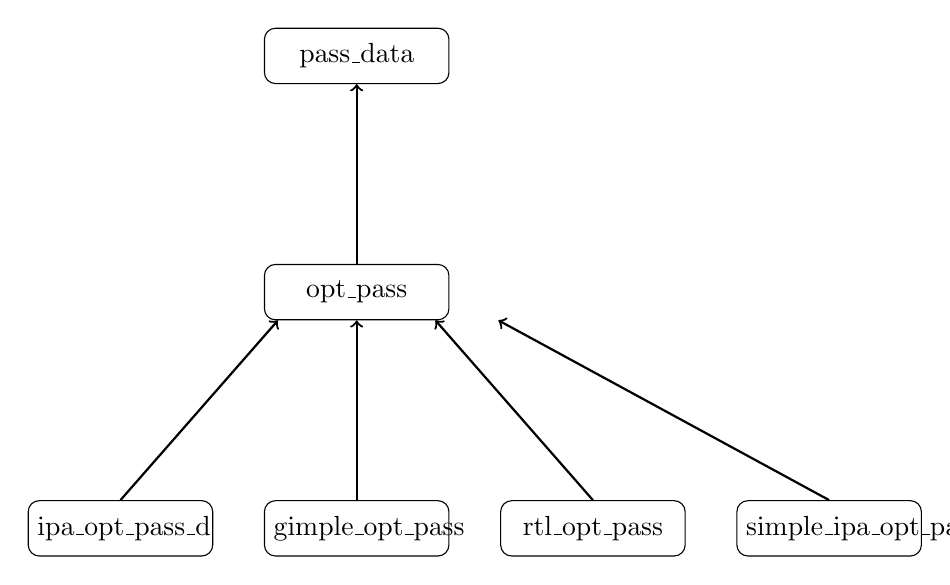
\begin{tikzpicture}[node distance = 5cm, auto]
    % Place nodes
    \node [block]                         (pass_data)   {pass\_data};
    \node [block, below of=pass_data]     (opt_pass) {opt\_pass};

    \node [block, below of=opt_pass]        (gimple_opt_pass) {gimple\_opt\_pass};
    \node [block, left of=gimple_opt_pass] (ipa_opt_pass_d)  {ipa\_opt\_pass\_d};
    \node [block, right of=gimple_opt_pass]  (rtl_opt_pass)    {rtl\_opt\_pass};
    \node [block, right of=rtl_opt_pass]    (simple_ipa_opt_pass) {simple\_ipa\_opt\_pass};

    % Draw edges
    \draw[->, thick]    (opt_pass.north)          -- (pass_data.south);

    \draw[->, thick]    (gimple_opt_pass.north)      -- (opt_pass.south);
    \draw[->, thick]    (ipa_opt_pass_d.north)       -- ([xshift=-1cm]opt_pass.south);
    \draw[->, thick]    (rtl_opt_pass.north)         -- ([xshift=1cm]opt_pass.south);
    \draw[->, thick]    (simple_ipa_opt_pass.north)  -- ([xshift=1.8cm]opt_pass.south);


\end{tikzpicture}
}
\end{center}
\caption{Hierarquia dos passos de otimização do GCC.}
\label{fig:opt_uml}
\end{figure}


\end{subsection}

%    Para realizar otimizações considerando as interações entre as rotinas,
%é utilizado um grafo de chamada de funções (\texttt{cgraphs}). Aqui as rotinas são
%representadas como um vértice no grafo, e existe um arco de $f$ à $g$
%quando há uma chamada de $g$ a partir de $f$. Dependendo da linguagem de
%programação utilizada, construir tais grafos pode ser uma tarefa simples pois
%as chamadas são especificadas estaticamente, como é o caso de Fortran; mas
%isto pode se tornar algo extremamente complexo quando orientação à objetos é
%empregada, pois é possível sobrescrever métodos.
%
%    Os grafos de chamadas de funções permitem otimizações que eliminem chamadas
%de funções, economizando assim o custo da chamada, e ainda permitem com que as
%funções sejam emitidas por ordem de proximidade, evitando com que o salto no
%fluxo de execução seja demasiado longo, o que implicaria em \textit{cache miss}.
%Também é possível propagar informações a respeito de outras funções, por exemplo
%propagar que uma certa função não altera um estado global ou interno desta
%(e.g. imprimir na tela, alterar um objeto), e em seguida calcular o resultado
%desta em tempo de compilação e remover sua chamada. Isto permite binários menores
%e código mais rápido, pois evita a necessidade de computar valores em tempo de
%execução.
%

%Um exemplo é o \textit{Register Transfer Language} (RTL) onde o código é
%representado como uma sequência de instruções em uma máquina de infinitos
%registradores. 

\begin{subsection}{GNU Toolchain e o Processo Clássico de Compilação}

    Um \textit{toolchain} é um conjunto de ferramentas que são ligadas em
uma cascata para o desenvolvimento de \textit{software}. Normalmente o
\textit{toolchain} consiste em um compilador, um montador e um linkeditor,
mas também pode conter mais ferramentas, como um \textit{debugger}.

A GNU providencia um conjunto de ferramentas para desenvolvimento de software
conhecido como GNU \textit{toolchain}. São parte desse toolchain:
\begin{itemize}
    \item \textit{Binutils}, um conjunto de ferramentas contendo o linkeditor
LD, o montador AS, e outras ferramentas\footnote{\url{https://www.gnu.org/software/binutils/}}.

    \item O driver \texttt{gcc}, providenciando os compiladores \texttt{cc1},
        \texttt{cc1plus}, \texttt{f951} para C, C++ e Fortran, respectivamente,
        e responsável por chamar as ferramentas do \textit{Toolchain}.

    \item A biblioteca \texttt{glibc}.

    \item O \textit{debugger} GDB.
\end{itemize}

As ferramentas acima interagem umas com as outras da seguinte forma: Primeiro, o código na
Linguagem Fonte é compilado usando o GCC para a linguagem de máquina. Em seguida, o código
é montado utilizando o AS, onde é construído um arquivo objeto, para que então o linkeditor
LD colete todos os arquivos objetos gerados, gerando o binário especificado. A Figura
\ref{fig:gnu_toolchain} retrata esse processo.


\begin{figure}
\tikzstyle{block} = [rectangle, draw, fill=white,
    text width=6em, text centered, rounded corners, node distance=6.5cm, auto, minimum height=2em]
\tikzstyle{line} = [draw, -latex]
\tikzstyle{cloud} = [draw, ellipse,fill=white, node distance=2cm,
    minimum height=2em]
\begin{center}
\scalebox{0.7}{
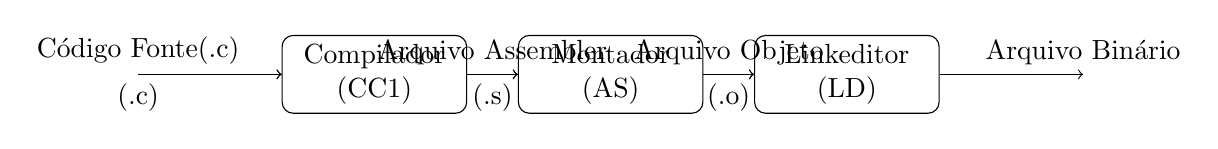
\begin{tikzpicture}[node distance = 3cm, auto]
    % Place nodes
    \node [block]                      (cc1) {Compilador \\ (CC1)};
    \node [block, right of = cc1]      (as) {Montador\\(AS)};
    \node [block, right of = as]       (ld) {Linkeditor\\(LD)};
    \coordinate [left of=cc1]          (fonte);
    \coordinate [right of=ld]    (bin);

    % Draw edges
    \draw[->]    (cc1.east)    -- (as.west)       node[midway, above] {Arquivo Assembler};
    \draw[->]    (cc1.east)    -- (as.west)       node[midway, below] {(.s)};
    \draw[->]    (as.east)     -- (ld.west)       node[midway, above] {Arquivo Objeto};
    \draw[->]    (as.east)     -- (ld.west)       node[midway, below] {(.o)};
    \draw[->]    (fonte.west)  -- (cc1.west)      node[pos=0, above] {Código Fonte\\ (.c)};
    \draw[->]    (fonte.west)  -- (cc1.west)      node[pos=0, below] {(.c)};
    \draw[->]    (ld.east)     -- (bin.west)      node[pos=1, above] {Arquivo Binário};
\end{tikzpicture}
}
\end{center}
\caption{Etapas de Compilação.}
\label{fig:gnu_toolchain}
\end{figure}

Esse processo é tradicionalmente usado para compilar \textit{softwares} complexos,
em conjunto com uma ferramenta que controla a geração de arquivos objetos e executáveis
como o GNU Make, como ilustrado na Figura \ref{fig:classical_build}. Aqui cada arquivo
é compilado individualmente, passando por todos os processos da compilação (tradução
para a linguagem intermediária, otimização, tradução para a Linguagem Alvo,
e encapsulamento no arquivo objeto), para em seguida eles sejam ligados por um
linkeditor como o LD. Aqui nenhuma otimização é aplicada observando o programa
como um todo, ou como as funções interagem entre si entre dois arquivos distintos,
gerando possivelmente um código suboptimal. Usualmente, cada um desses arquivos
são compilados em paralelo através do auxilio do Makefile.



\begin{figure}
\tikzstyle{block} = [rectangle, draw, fill=white,
    text width=6em, text centered, rounded corners, node distance=3cm, auto, minimum height=2em]
\tikzstyle{line} = [draw, -latex]
\tikzstyle{cloud} = [draw, ellipse,fill=white, node distance=2cm,
    minimum height=2em]
\begin{center}
\scalebox{0.7}{
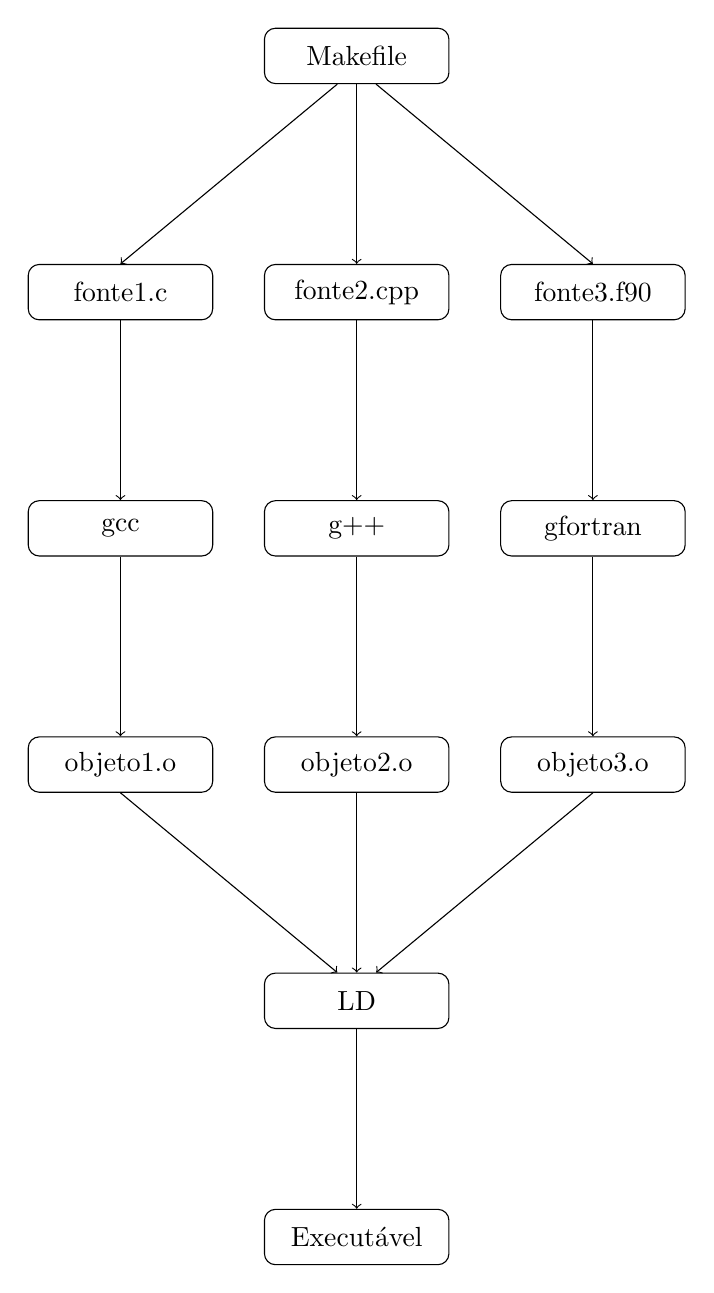
\begin{tikzpicture}[node distance = 3cm, auto]
    % Place nodes
    \node [block]                         (make)   {Makefile};
    \coordinate[below of=make]            (c);
    \node [block, left of=c]              (fonte1) {fonte1.c};
    \node [block, right of=fonte1]        (fonte2) {fonte2.cpp};
    \node [block, right of=fonte2]        (fonte3) {fonte3.f90};

    \node [block, below of=fonte1]        (gcc)      {gcc};
    \node [block, below of=fonte2]        (g++)      {g++};
    \node [block, below of=fonte3]        (gfortran) {gfortran};

    \node [block, below of=gcc]           (objeto1) {objeto1.o};
    \node [block, below of=g++]           (objeto2) {objeto2.o};
    \node [block, below of=gfortran]      (objeto3) {objeto3.o};

    \node [block, below of=objeto2]       (ld) {LD};

    \node [block, below of=ld]            (bin) {Executável};

    % Draw edges
    \draw[->]    ([xshift=-0.7em] make.south)   -- (fonte1.north);
    \draw[->]    (make.south)   -- (fonte2.north);
    \draw[->]    ([xshift=+0.7em] make.south)   -- (fonte3.north);

    \draw[->]    (fonte1.south)   -- (gcc.north);
    \draw[->]    (fonte2.south)   -- (g++.north);
    \draw[->]    (fonte3.south)   -- (gfortran.north);

    \draw[->]    (gcc.south)   -- (objeto1.north);
    \draw[->]    (g++.south)   -- (objeto2.north);
    \draw[->]    (gfortran.south)   -- (objeto3.north);

    \draw[->]    (objeto1.south)   -- ([xshift=-0.7em]ld.north);
    \draw[->]    (objeto2.south)   -- (ld.north);
    \draw[->]    (objeto3.south)   -- ([xshift=+0.7em]ld.north);

    \draw[->]    (ld.south)   -- (bin.north);


\end{tikzpicture}
}
\end{center}
\caption{Processo clássico de compilação de um programa.}
\label{fig:classical_build}
\end{figure}


\end{subsection}

\end{section}

\begin{section}{Computação Paralela}
\label{sec:parallel_comp}

    A Computação Paralela é o ato de coordenar vários fluxos de
execução operando simultaneamente em um ou mais computadores para
atingir um objetivo em comum. Ela se tornou uma tendência na
computação contemporânea por conta dos processadores \textit{multicore}
e \textit{manycore}, que hoje podem ser adquiridos facilmente e são
produzidos com um custo menor do que um processador de apenas um
núcleo de igual desempenho.

    Para ilustrar a evolução dos processadores \textit{multicore}, \cite{42years}
    publicou um gráfico mostrando o número
de transistores, núcleos e desempenho de cada núcleo desde 1970,
apresentado na Figura \ref{fig:42years}.
Neste gráfico é possível notar que a Lei de Moore ainda se aplica,
mas a desempenho sequencial dos processadores estão em desaceleração,
enquanto o número de núcleos cresce exponencialmente desde 2008. Isto
justifica o uso de computação paralela sempre que possível para que
seja utilizado o máximo dos recursos computacionais disponíveis.

    Nessa seção são discutidas alguns conceitos básicos de computação
paralela e alguns algoritmos úteis na paralelização de programas.

\begin{figure}[ht]
 \centering
 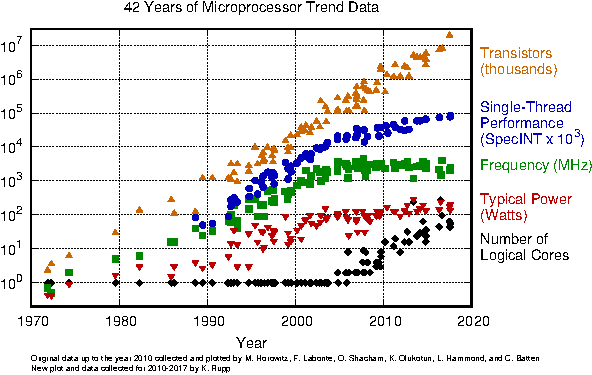
\includegraphics[scale=1.2]{42-years-processor-trend.pdf}
 \caption{42 anos de evolução dos processadores. Fonte: \cite{42years}}
 \label{fig:42years}
\end{figure}

\begin{subsection}{\textit{Speedup}}
    Uma maneira de medir o ganho de tempo em uma implementação paralela
de um algoritmo é através no conceito de \textit{speedup}. Sejam $T_1$
o tempo do algoritmo sequencial e $T_n$ o tempo desse algoritmo paralelizado
    com $n$ núcleos de processamento. Então o \textit{speedup} $S_n$
é dado por:
    $$ S_n = \frac{T_1}{T_n} $$

\end{subsection}


\begin{subsection}{A Taxonomia de Flynn}
	Mesmo com a evolução dos processadores \textit{multicore} e
\textit{manycore}, esses não são as únicas arquiteturas disponíveis para
realizar computação paralela.  Michael J. Flynn \citep{pacheco:2011} definiu
uma taxonomia das arquiteturas, mas vale destaque para duas delas:
\begin{enumerate}
    \item \textbf{SIMD} - \textit{Single Instruction, Multiple Data}. Isso se refere
        a processadores vetoriais que permite com que uma operação seja executada em
        todos os elementos de um vetor simultâneamente. Alguns exemplos são as
        instruções SSE da Intel, e também as \textit{Graphics Processing Units} (GPU),
        embora essa última não seja considerada uma arquitetura puramente SIMD.

    \item \textbf{MIMD} - \textit{Multiple Instruction, Multiple Data}. Isso se refere
        aos sistemas \textit{multicore} independentes, capazes de executar tarefas
        de maneira assíncrona. Aqui estão localizados ambas as arquiteturas de memória
        compartilhada e memória distribuida.
\end{enumerate}
\end{subsection}

\begin{subsection}{Programação Paralela em Memória Compartilhada}
	Uma maneira de permitir Computação Paralela é através de
uma memória compartilhada. Aqui vários processadores ou núcleos
são ligados através de um barramento a uma memória compartilhada entre
todos os processadores, que permite leitura e escrita de dados.
Para evitar problemas de concorrência, são necessários mecanismos de
travas e sincronização.

	 Aqui, muitos dos recursos para sincronização são fornecidos pelo
Sistema Operacional (OS), e portanto é necessário explicar um pouco
das abstrações que ele fornece.

\begin{subsubsection}{Processos e \textit{Threads}}

	Antigamente, os processadores eram capazes de executar apenas
um programa por vez. Com isto em mente, os desenvolvedores
de Sistemas Operacionais criaram uma série de abstrações para que fosse
possível dar a ilusão ao usuário que vários programas estavam executando
ao mesmo tempo. Embora isso não seja mais um fato já que hoje os processadores
são capazes de executar vários fluxos de execução simultaneamente, essa
é a principal motivação do conceito de Processos e \textit{Threads}.

	Um \textit{Processo} é um modelo de abstração do Sistema Operacional que
dá a um programa a ilusão de que ele tem o monopólio do processador
\citep{love:2005}. Cada processo tem a sua região de memória privada por
padrão, e para que processos possam compartilhar memória, isso deve ser 
explicitado no programa. Um exemplo onde isso pode ser feito é através das
chamadas \texttt{shmget} do extinto \texttt{System V}, mas cujo o Linux ainda
oferece suporte \citep{shmget}.

Cada processo contém pelo menos um fluxo de execução, e cada fluxo de
execução é chamado de \textit{thread}. Cada \textit{thread} dentro
de um processo compartilha memória com as demais \textit{threads}
do processo, facilitando assim o desenvolvimento de mecanismos de
comunicação através de uma memória compartilhada.

\end{subsubsection}

\begin{subsubsection}{Mecanismos de Sincronização}

	Seja através de auxílio de \textit{hardware}, ou com algoritmos
puramente implementados em \textit{software}, o Sistema Operacional
costuma fornecer mecanismos de sincronização para coordenar as várias
\textit{threads} de um processo, ou até mesmo vários processos.

    Um dos mecanismos mais famosos são os \textit{Semáforos}
\citep{dijkstra1965}.  Um semáforo nada mais é que um contador que assume
valores não negativos com duas operações atômicas: \texttt{P} para
decrementá-lo, e \texttt{V} para incrementá-lo. Quando o semáforo atinge o
valor 0, a \textit{thread} que em sequência tentar decrementá-lo será bloqueada. A
sua execução apenas será retomada quando o semáforo for novamente incrementado
por outra \textit{thread} \citep{semaphore}.

    Semáforos também podem ser utilizados para resolver o problema da
seção crítica, que é uma seção de código que apenas uma \textit{thread}
deve poder executar por vez, embora seja mais comum a utilização
de \textit{Mutexes}.

\textit{Mutexes} nada mais são que uma estrutura que garante a exclusão
mútua de uma região, conforme ilustrado na Figura \ref{fig:mutex}. Nessa
figura, três \textit{threads} são iniciadas executando a função $f$, mas
apenas uma pode executar a seção crítica.
    Quando o \textit{mutex} \texttt{lock} é travado,
todas as outras \textit{threads} que tentarem acessar a seção crítica
serão bloqueadas pelo Sistema Operacional, garantindo assim que apenas
uma \textit{thread} esteja executando a seção crítica.
As \textit{threads} bloqueadas somente voltarão a executar quando o
    \textit{mutex} for desbloqueado pela \textit{thread} que o travou.
\begin{figure}
      \begin{lstlisting}[
        language=pseudocode,
        style=pseudocode,
        style=wider,
        functions={},
        specialidentifiers={extern, call, async, mutex_t},
      ]
        extern function mutex_lock, mutex_unlock;
        mutex_t lock;

        async function f()
            mutex_lock(lock);
                // Região crítica
            mutex_unlock(lock);
        end

        function main()
            for i=1, 3 do
                call f;
            done
        end
      \end{lstlisting}
      \caption{Ilustração de uso de um mutex,}
      \label{fig:mutex}
\end{figure}

Outro mecanismo de sincronização muito útil são as Barreiras. Uma barreira
é um ponto no programa onde, assim que a \textit{thread} o executar, ela
será bloqueada até que todas as \textit{threads} cheguem ao mesmo ponto, como
ilustrado na Figura \ref{fig:barrier}.
Isso é bastante útil para evitar que uma \textit{thread} avance na execução
do código enquanto ela deveria estar aguardando o resultado da computação
de outras \textit{threads}. As barrerias também costumam receber um parâmetro
de inicialização indicando quantas \textit{threads} precisam atingir a
barreira para que todas as \textit{threads} que a atingiu sejam desbloqueadas.

\begin{figure}[ht]
 \centering
 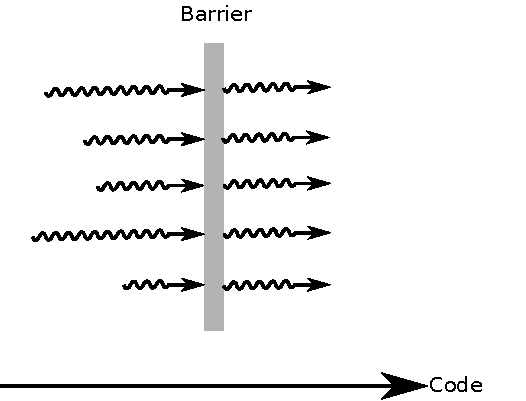
\includegraphics[scale=1.0]{barrier.pdf}
 \caption{Ilustração do funcionamento de uma barreira.}
 \label{fig:barrier}
\end{figure}


Por fim, exceto os semáforos, todos esses mecanismos mencionados acima são
implementados na biblioteca \texttt{Pthread}. Já os semáforos estão disponíveis
no Linux através da interface \texttt{semaphore.h}.

\end{subsubsection}

\begin{subsubsection}{O Problema do Produtor-Consumidor}
    Uma estrutura de dados muito útil em computação paralela
é uma fila que seja completamente \textit{Thread-safe}, ou seja,
que várias \textit{threads} possam inserir e remover dados dessa
fila simultaneamente sem o risco de perda de dados. Essa fila
pode ser usada na comunicação entre as \textit{threads}, por
exemplo, uma insere trabalho na fila, outra retira trabalho da
fila. Isso permite com que \textit{pipelines}, ou escalonamento
dinâmico de trabalho, sejam implementados.

Para implementar essa fila, são necessários dois semáforos e um
\textit{mutex}. Um semáforo deve ser inicializado com o tamanho máximo
da fila, e na inserção de um dado, esse semáforo deve ser decrementado
para que quando a fila estiver cheia, as \textit{threads} que tentarem
inserir nela sejam bloqueadas. O outro semáforo deve ser iniciado com
0, indicando que a fila está vazia, e incrementado quando um item for
inserido na fila. Esse semáforo tem a finalidade de
bloquear as \textit{threads} que tentarem remover elementos dessa
fila quando ela estiver vazia. Assim que dados forem inseridos ou removidos
da fila, as \textit{threads} são devidamente acordadas. Isso evita gasto
desnecessário de ciclos de processamento, evitando utilizar uma técnica
chamada \textit{espera ocupada}. Por fim, um \textit{Mutex} deve ser
utilizado para evitar problemas de concorrência ao incrementar e
decrementar os apontadores de inicio e fim da fila. Uma implementação
está apresentada na Figura \ref{fig:prod_consumer}.

\begin{figure}
      \begin{lstlisting}[
        language=pseudocode,
        style=pseudocode,
        style=wider,
        functions={},
        specialidentifiers={extern, call, async, int, class, mod, semaphore_t, mutex_t},
      ]
        class Fifo
            int buffer[];
            int size;
            int head, tail;
            semaphore_t full, empty;
            mutex_t lock

            function init(n)
                buffer = allocate_memory(n);
                head, tail = 0;
                sem_init(empty, n);
                sem_init(full, 0);
                mutex_init(lock);
                size = n;
            end

            function push(element)
                sem_p(empty);
                mutex_lock(lock);
                buffer[head] = element;
                head = head + 1 mod size;
                mutex_unlock(lock);
                sem_v(full);
            end

            function pop()
                sem_p(full);
                mutex_lock(lock);
                ret = buffer[tail];
                tail = tail + 1 mod size;
                mutex_unlock(lock);
                sem_v(empty)

                return ret;
            end
        end 

      \end{lstlisting}
      \caption{Uma implementação do Produtor-Consumidor.}
      \label{fig:prod_consumer}
\end{figure}

\end{subsubsection}

\end{subsection}

\end{section}
